	\psset{xunit=1.2cm,yunit=1.2cm,labelFontSize=\scriptstyle,showorigin=false}
	\begin{pspicture}(-1,-1.4)(10.5,3.7)
		\multido{\n=-0.2+0.2}{56}{\psline[linewidth=0.35pt,linecolor=lightgray](\n,-1)(\n,3)}
		\multido{\n=-1.0+0.2}{21}{\psline[linewidth=0.35pt,linecolor=lightgray](0,\n)(10.8,\n)}
		\multido{\n=0+1}{11}{\psline[linewidth=0.45pt](\n,-1)(\n,3)}
		\multido{\n=-1+1}{5}{\psline[linewidth=0.45pt](0,\n)(10.8,\n)}
		\psaxes[linewidth=0.95pt]{->}(0,0)(0,-1)(11,3)
		\def\Func{x 6 mul  2.71828 x exp div}
		\psplot[plotpoints=3000,linewidth=1.25pt,linecolor=red]{0}{10}{\Func}
		\uput[ur](2.5,1.5){\red $\mathcal{C}$}
	\end{pspicture}
	
	\subsection*{1.}
	La fonction \(f\) est un quotient de fonctions dérivables, le dénominateur étant non nul quel que soit le réel \(x\). On a donc sur \(\mathbb{R}\), et en particulier sur \([0\,;\,10]\) :
	\[
	f'(x) = \dfrac{6 e^x - 6x \times e^x}{(e^x)^2} = \dfrac{6 e^x (1 - x)}{e^x \times e^x} = \dfrac{6 (1 - x)}{e^x}.
	\]
	
	\subsection*{2.}
	Comme \(6 e^x > 0\) quel que soit \(x\), pour \(x \in [0\,;\,10]\), le signe de \(f'(x)\) est celui de \(1 - x\) :

		 \begin{align*}
		&1 - x > 0\\
		 \iff& 1 > x \\
		\iff& x < 1 
		\end{align*}
		La fonction \(f\) est donc croissante sur \([0\,;\,1]\), \\
		de \(f(0) = 0\) à \(f(1) = \dfrac{6 \times 1}{\e^1} = 6 \e^{-1} \approx 2,207\) ;
	
		\begin{center}
		\begin{tikzpicture}[double distance=2pt]
			\tkzTabInit{$x$/1,f'(x)/1,$f(x)$/2}{$0$,$1$, $10$}
			\tkzTabLine{,+,z, -}
			\tkzTabVar{+/$0$,-/ $6\e^{-1}$ /, +/}
		\end{tikzpicture}
	\end{center} 
	\subsection*{3.}
	Les variations de \(f\) montrent que la concentration maximale est atteinte après 1 heure et qu'elle est égale à environ \(2,2\) (mg/L).
	
	\subsection*{4.}
	Le sportif peut être contrôlé à tout moment après son injection, mais hélas il sera en infraction entre environ 43 minutes et 1h24 après l'injection car la concentration sera à ce moment supérieure à \(2\) (mg/L).
	
